\chapter{Software Implementation and System Architecture}
\label{chap:implementation}

\section{System Architecture Overview}
The software architecture of the \textbf{Quantum Resource Optimizer} is organized within the package directory \texttt{src/quantum\_optimizer/}. The design enforces a strict separation of concerns between domain data structures, classical baseline algorithms, quantum Hamiltonian compilation, variational circuit execution, experiment orchestration, and data visualization.

\begin{figure}[htbp]
    \centering
    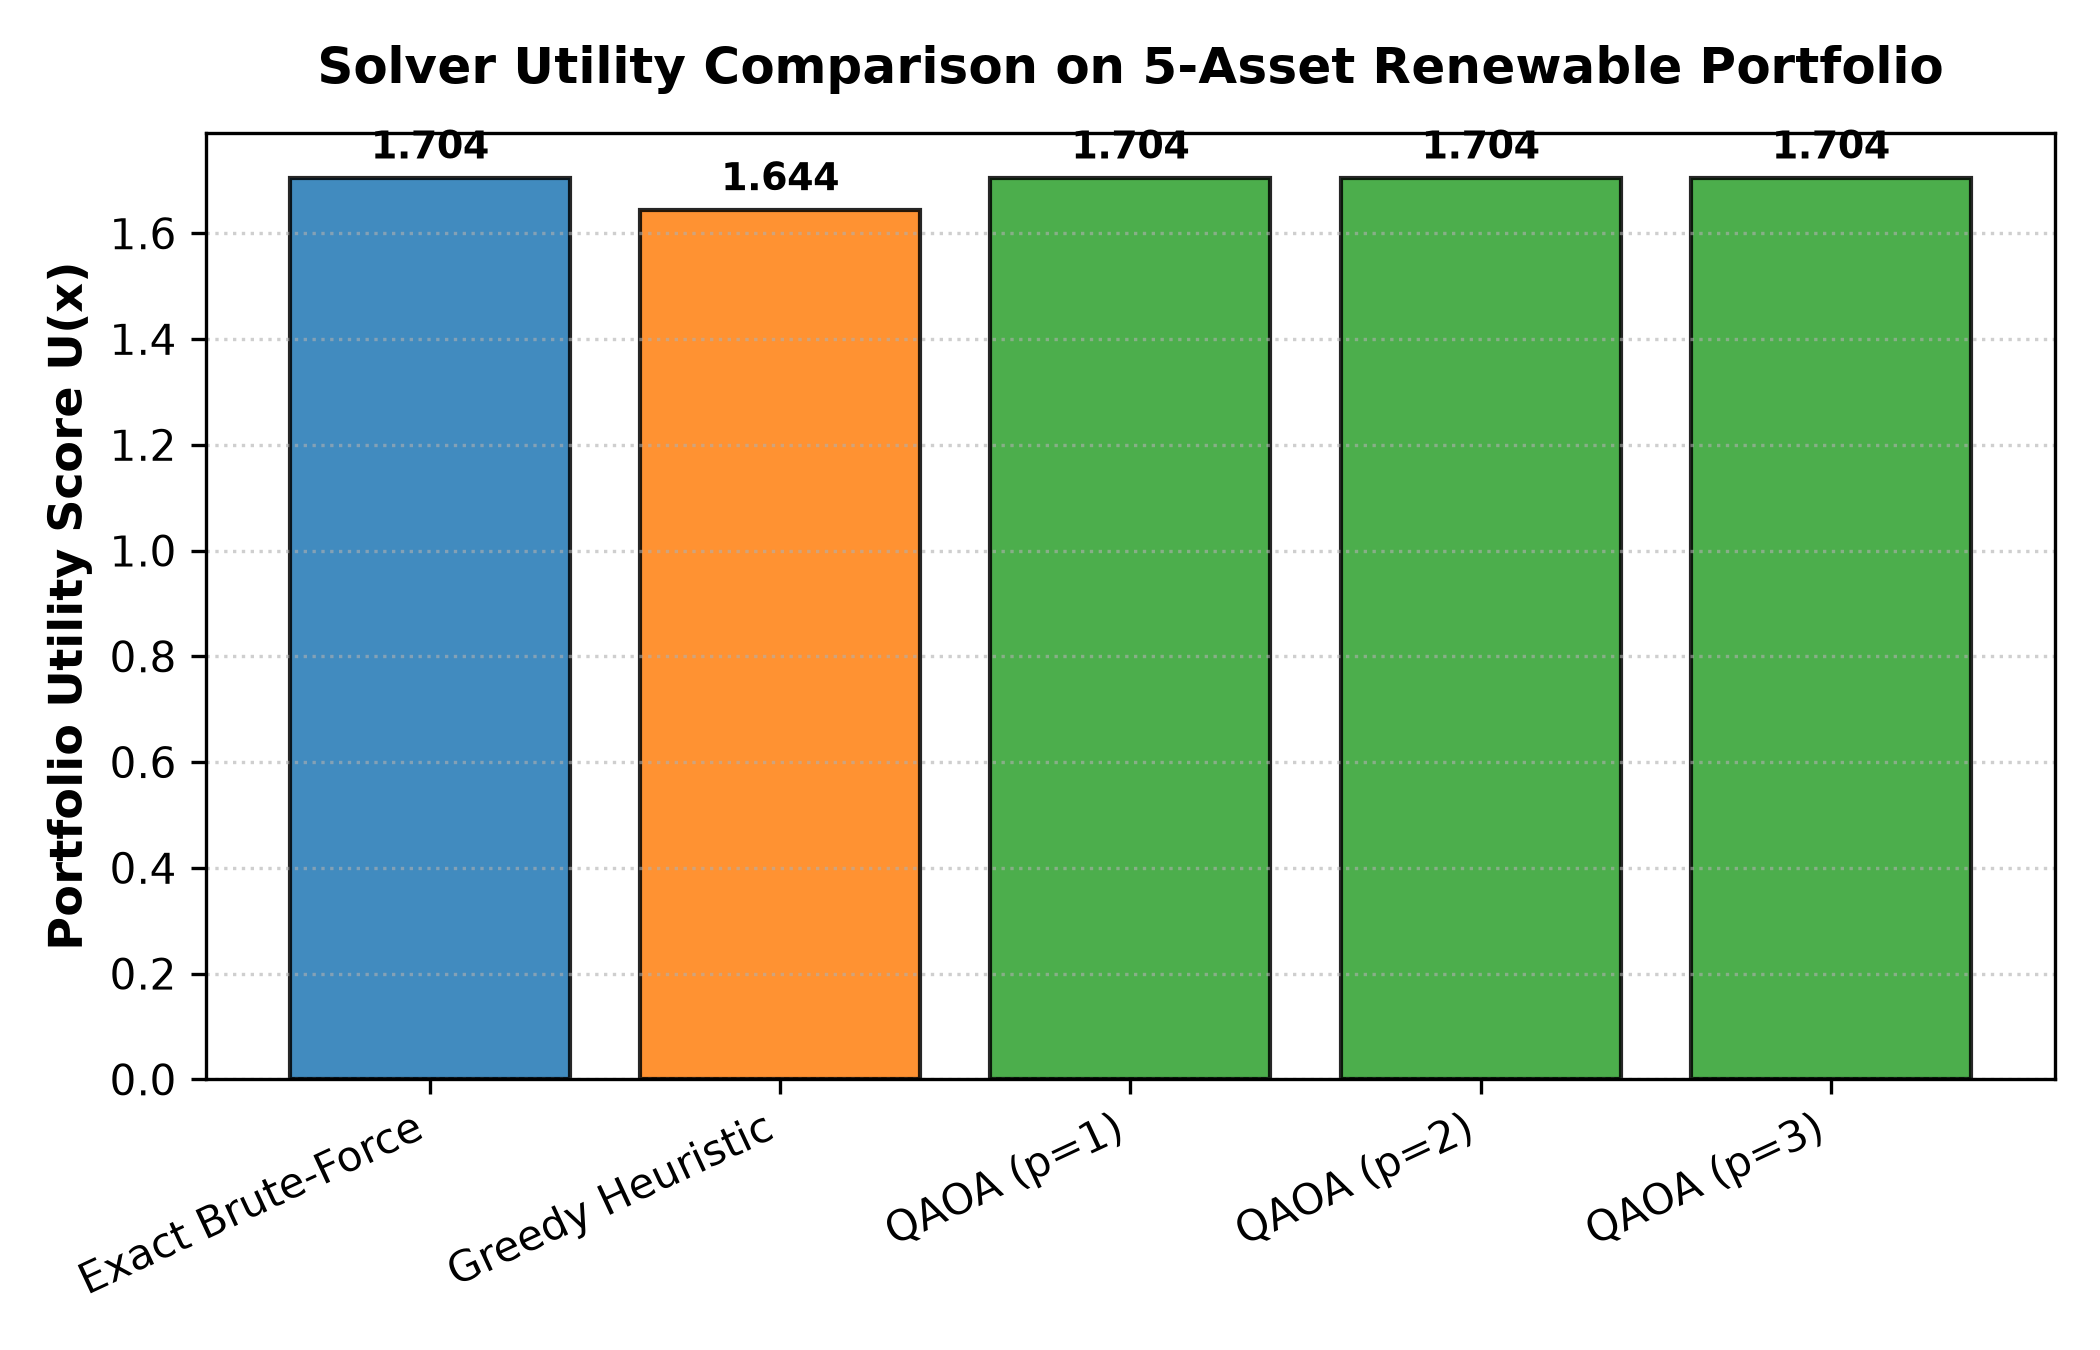
\includegraphics[width=0.8\textwidth]{figures/solver_utility_comparison.png}
    \caption{Comparative solver utility across candidate portfolios, contrasting the exact global optimum, the classical greedy choice, and the QAOA candidate distribution.}
    \label{fig:solver_utility}
\end{figure}

\section{Core Modules and Interfaces}
The codebase is structured into six modular components:

\subsection{\texttt{problem.py}: Domain Modeling and Validation}
Encapsulates problem data and mathematical evaluation logic.
\begin{itemize}
    \item \texttt{Asset}: An immutable data class storing asset index, descriptive name, technology category, expected generation return $r_i$, and annual carbon offset.
    \item \texttt{ProblemInstance}: Stores the asset catalog, return vector $r \in \mathbb{R}^N$, covariance matrix $\Sigma \in \mathbb{R}^{N \times N}$, budget cap $B$, risk factor $q$, and penalty weight $\lambda$.
    \item \texttt{validate()}: Enforces domain constraints: $N \ge 2$, $1 \le B < N$, $q \ge 0$, $\lambda > 0$, matrix symmetry $\Sigma = \Sigma^\top$, and shape consistency.
    \item \texttt{evaluate\_utility(x)}: Computes the Markowitz objective $\mathcal{U}(x) = r^\top x - \frac{q}{2} x^\top \Sigma x$.
    \item \texttt{evaluate\_cost(x)}: Computes the unconstrained scalar cost $C(x) = -\mathcal{U}(x) + \lambda (\sum_i x_i - B)^2$.
    \item \texttt{is\_feasible(x)}: Verifies whether $\sum_i x_i = B$.
\end{itemize}

\subsection{\texttt{classical\_solvers.py}: Ground Truth and Heuristic Baselines}
Provides deterministic benchmarks for validating quantum performance:
\begin{itemize}
    \item \texttt{BruteForceSolver}: Iterates exhaustively through all $2^N$ binary bitstrings, scoring both cost $C(x)$ and utility $\mathcal{U}(x)$ for every state. It identifies the provable global optimum $x^*$, serving as the absolute benchmark for approximation ratio calculation.
    \item \texttt{GreedyHeuristicSolver}: Implements a fast classical greedy selection. It sorts assets in descending order of individual net utility $u_i = r_i - \frac{q}{2}\Sigma_{ii}$ and selects the top $B$ assets. Crucially, this heuristic ignores pairwise covariance interactions $q \Sigma_{ij}$ ($i \neq j$), providing a realistic baseline for scenarios where cross-asset risks are neglected.
\end{itemize}

\subsection{\texttt{hamiltonian.py}: Algebraic QUBO and Ising Compilation}
Implements the transformation from the mathematical model to Qiskit quantum operators:
\begin{itemize}
    \item \texttt{build\_qubo\_matrix(problem)}: Computes the diagonal coefficients $Q_{ii}$ and pairwise upper-triangular coefficients $Q_{ij}$ according to Equations \eqref{eq:q_diag} and \eqref{eq:q_ij}.
    \item \texttt{build\_cost\_hamiltonian(problem)}: Converts QUBO terms into a Qiskit \texttt{SparsePauliOp} by evaluating the exchange couplings $J_{ij}$ and local fields $h_i$. Qiskit's native Pauli string representation orders qubit $k$ at position $(n - 1 - k)$ from left to right.
    \item \texttt{verify\_hamiltonian\_ground\_state(problem, hamiltonian)}: Extracts the diagonal of the full $2^N \times 2^N$ Hamiltonian matrix and asserts that $\langle x | \hat{H}_C | x \rangle == C(x)$ for all $2^N$ states within tolerance $\epsilon = 10^{-6}$.
\end{itemize}

\subsection{\texttt{qaoa\_solver.py}: Variational Execution and Bitstring Decoding}
Orchestrates Qiskit 2.5 primitives and post-processing:
\begin{itemize}
    \item Initializes \texttt{QAOAAnsatz(cost\_operator, reps=p)} with unmeasured and measured circuit variants.
    \item \texttt{optimize()}: Executes COBYLA iterations over the expectation value computed using \texttt{StatevectorEstimator}.
    \item \texttt{sample()}: Invokes \texttt{StatevectorSampler} on the measured ansatz to obtain categorical counts over 4096 shots.
    \item \texttt{key\_to\_assignment(key, n)}: Decodes and reverses the little-endian measurement key into asset assignment vectors.
    \item Computes final metrics: Approximation Ratio $\alpha$, Feasibility Yield $Y_{\text{feas}}$, optimizer iterations, and runtime.
\end{itemize}

\subsection{\texttt{experiment\_runner.py}: Multi-Parameter Sweeps}
Automates reproducible experiment execution, recording configuration metadata, git commit hash, environment versions, and full metric histories to structured JSON and CSV artifacts under \texttt{outputs/runs/}.

\subsection{\texttt{visualization.py}: Publication Graphics Generation}
Generates high-resolution publication plots (Figures \ref{fig:qaoa_circuit}, \ref{fig:solver_utility}, \ref{fig:convergence}, \ref{fig:distribution}, \ref{fig:depth_scaling}, and \ref{fig:penalty_sweep}) formatted with Seaborn/Matplotlib styling.

\section{Automated Verification Suite}
The codebase includes an automated test suite executed via \texttt{pytest tests/}:
\begin{itemize}
    \item \texttt{test\_problem\_validation}: Validates rejection of non-symmetric covariance matrices, invalid budget values ($B \ge N$, $B \le 0$), negative risk factors, and non-positive penalties.
    \item \texttt{test\_qubo\_and\_hamiltonian\_equivalence}: Formally verifies that $\langle x | \hat{H}_C | x \rangle \equiv C(x)$ across all 32 basis states.
    \item \texttt{test\_classical\_solvers}: Confirms that brute force identifies the true minimum cost and that the greedy solver returns a feasible bitstring with $\sum x_i = B$.
    \item \texttt{test\_qaoa\_endianness\_and\_decoding}: Verifies that little-endian bitstring keys from Qiskit map bijectively to the correct asset indices.
    \item \texttt{test\_qaoa\_solver\_execution}: Runs an end-to-end QAOA optimization on a 3-asset toy instance, asserting that the approximation ratio exceeds 0.90 and execution terminates cleanly.
\end{itemize}
All 12 test assertions pass in 2.22 seconds on the local Python 3.12 virtual environment.
